\documentclass[9pt,twocolumn,twoside]{pnas-report}

\templatetype{pnasresearcharticle}

\usepackage{lipsum}

\title{Effect of Key Match Events on Football Passmaps}

\author[a,1]{Vid Stropnik}
\author[a]{Vuk \DJ uranović}
\author[a]{Maruša Oražem} 


\affil[a]{University of Ljubljana, Faculty of Computer and Information Science, Ve\v{c}na pot 113, SI-1000 Ljubljana, Slovenia}


\leadauthor{Stropnik} 
\authordeclaration{All authors contributed equally to this work.}
\correspondingauthor{\textsuperscript{1}To whom correspondence should be addressed. E-mail: vs2658@student.uni-lj.si}





\begin{abstract}
\lipsum[1]
\end{abstract}

\dates{The manuscript was compiled on \today}
\doi{\href{https://ucilnica.fri.uni-lj.si/course/view.php?id=183}{Introduction to Network Analysis} 2020/21}

\begin{document}

\maketitle
\thispagestyle{firststyle}
\ifthenelse{\boolean{shortarticle}}{\ifthenelse{\boolean{singlecolumn}}{\abscontentformatted}{\abscontent}}{}



\dropcap{A}{\bf ssociation football is the world's most popular sport.} During gameplay, players attempt to create goal-scoring opportunities through various methods of individual control of the ball. While these can include dribbling, tackling and taking direct shots, the most common one is passing the ball to a teammate. Progressing the ball along the pitch with a series of passes helps the team retain control of the match, enabling them to realize set plays. It is worth noting that this method is not only common, but also effective, as exhibited by the correlation of per-game average pass frequency and overall tea, success. \cite{plpasses}

Ball movement and goal-scoring opportunities in a football match are complex phenomena to model. Pass characteristics, such as their length, speed or the involved players' positions are often used to provide further insights into their importance and quality. Logging such characteristics for hundreds of passes that happen in any given football match, however, renders the resulting data structure very complex and hard to interpret. To infer more general information about longer stints of play, simpler arrangements, such as networks with player nodes and directed pass links, should be considered.

There are several events in any given football match, that might incur a fundamental change in a team's tactics and approach towards the game. The coaching staff might recognize weak points in the opposition's strategy and relay them to the players during half-time. Suddenly conceding a goal in a must-win game might prompt a team to take more risks and try a different approach, while we can often observe leading teams resort to time-wasting tactics to ensure their victory. 

In this course project, we introduce novel ways of football match analysis using established network science approaches. By using methods of measuring change in team pass map centrality, by observing alterations of its underlying communities and by recognizing the (dis)appearance of distinct player graphlets as a result of a key event in a football match, we study common team behaviours that key match events might induce. We recognize these insights as useful in several areas. First, they serve as a form of establishing several ground truths about common trends of play, that will underpin further research. Secondly, more fine-grained difference of successful and unsuccessful responses to key events might be observed and be used in match preparations by domain experts. Finally, we recognize real-time applications of the proposed methods as useful in broadcasting, betting, commentary and analytics, to name only a few fields.

This report is structured as follows: In the following paragraphs, we provide a brief overview of the work, relating to inferring insights from sports data using network analysis. Here, we also introduce some key academic contributions to our work in the tree network science fields of special interest: measuring centrality, detecting communities and gathering semantic information from network graphlets. A subsection corresponds to each of these fields in the succeeding \textit{Results} section. In them, we introduce the main revelations about the effects of key match events on passing trends. We later comment on the implications of these results and asses their appropriateness for further application, while finally introducing our detailed methodologies at the end of the paper.



%\begin{figure}[t]\centering%
%	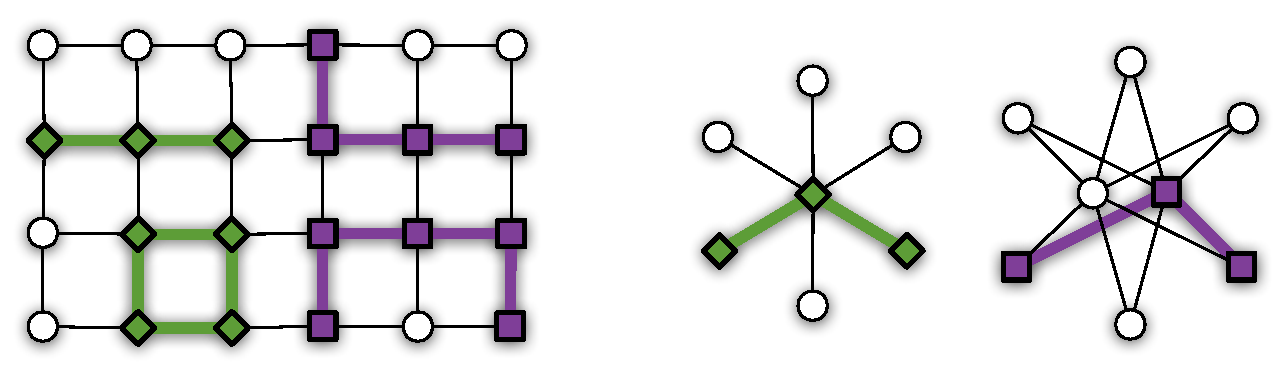
\includegraphics[width=0.8\linewidth]{examples}
%	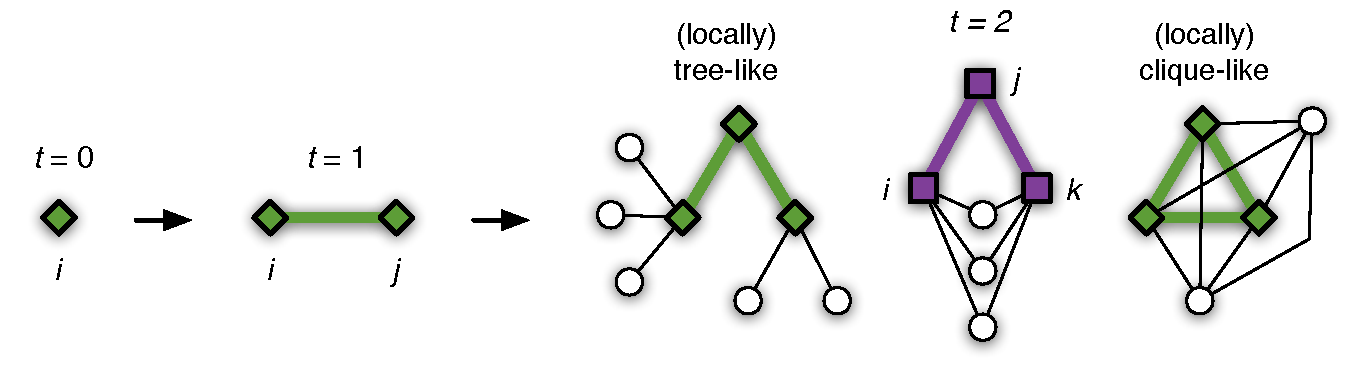
\includegraphics[width=\linewidth]{growth}
%	\caption{Mandatory informative illustration highlighting main %contributions.~\cite{Sub18a}}
%	\label{fig:example}
%\end{figure}

\section*{Related work}
Evaluations of group performances based on their underlying network structures have been conducted for some time. Researchers were keen on understanding what kind of social, interaction or communication network structure boosts the productivity of a group in a working environment. Bavelas \cite{bavelas} was one of the pioneers in exploration of information transfer between groups. He discovered that the rate of information diffusion was significantly smaller in decentralized networks in comparison to centralized ones. It was later discovered by Shaw \cite{shaw} that this gave an edge to decentralized groups over the centralized ones in solving complex tasks. \

Team performance in collective sports has become a well researched area in the network analysis community in recent years. We recognize the conclusions by Grund \cite{grund} as a good starting point for the study of this field. In his work, he suggests that small networks (i.e. the eleven-node football team) are better explained with the use of the weighted edges between players. In such cases, weights are determined by the frequency of passes between two players. He also introduces a measure called network intensity, as a counterpart to network density in large and unweighted networks. This measure is computed as a function of weights for each link between players, nicely called passing-rate of the team. As a result of his work, Grund confirmed that an increase in team passing rate leads to increased performance, while increases in centralization of play reduces team performance. A similar approach in generating a football passmap as a weighted network was used in \cite{fbrn}, where the authors introduced a node measure called flow centrality - a function of pass accuracy and ratio of times a player was included in an action, leading to a shot on goal. Using it, they successfully graded individual player performances within a team. Due to advances in player-tracking technology, most recent research, such as those by Fernandez and Born \cite{fbrn}, or by Chawla et al \cite{chawla}, exploits the spatial-temporal data about observed passes. Due to the restrictions posed by our course project, we don't expect to consider these additional pieces of information, but will instead focus on the starting formation of the team in determining the position of the player. Should we recognize the aspect of temporal network analysis as important throughout our work, however, work by Mattson and Takes \cite{trajectory} on pass trajectory extraction, should be considered.

\section*{Results}

\begin{table}[t]\centering%
	\caption{Table describing data or methods.}
	\begin{tabular}{lccccc}\toprule
	    & $n$ & $m$ & $\langle k\rangle$ & $\langle C\rangle$ & $\langle d\rangle$ \\\midrule
	    Fine network & $438\,920$ & $9\,742\,733$ & $44.4$ & $0.37$ & $6.19$ \\
	    Random graph & $438\,920$ & $9\,781\,609$ & $44.6$ & $0.00$ & $4.92$ \\\bottomrule
	\end{tabular}
	\label{tbl:example}
\end{table}

{\bf Main results supported by plots, figures, tables, diagrams etc.}
\lipsum[1-2]



\lipsum[3-8]

\section*{Discussion}

{\bf Discussion of results, main contributions, final conclusions and future work.}
\lipsum[1-5]

{\small\section*{Methods}

{\bf Describe data, methods and algorithms (use subsections).}
\lipsum[1-3]
\begin{equation}
	\phi_v = \Pr(X_{st}(v) = 1) = \Pr(X_{sv} = 1)\Pr(X_{vt} = 1)
	\label{eq:example}
\end{equation}

\lipsum[4-5]}

\acknow{The authors would like to\dots}

\showacknow{}

\bibliography{bibliography}

\end{document}